\Exercise[number={16}]
A generalized linear model is used to describe the relationship between a
feature vector \(x\) and an independent integer variable \(y\) that represents
the number of times an event occurs. The model is then defined by
\(z=b^T\cdot x\) where \(b\) is a vector of parameters, and \(y=f(z)\),
where \(f(...)\) is the output function. Prove that, if the observations
\(\hat{y}\) have a Poisson distribution, such as:
\begin{align*}
    p(\hat{y}|y)=\frac{e^{-y}\cdot y^{\hat{y}}}{\hat{y}!}
\end{align*}
then the canonical output function \(f(...)\) is the exponential.

\Answer[number={16}]
The drawing of the specified generalized linear model is the following one:
\begin{figure}[H]
    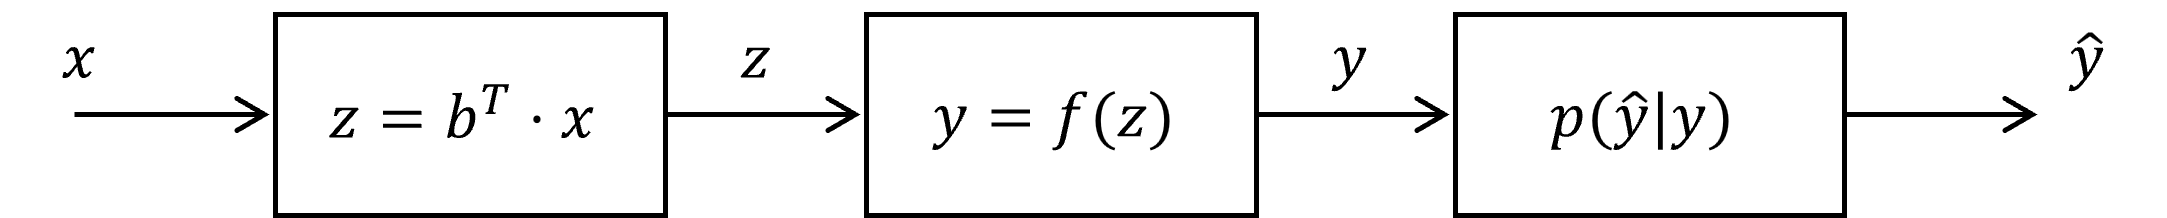
\includegraphics[scale=0.75]{C_16}
    \centering
\end{figure}
The dataset can be defined as \(D=\{(x_i, \hat{y_i}), i=1,...,N\}\), while
the likelihood is expressed as follow thanks to the chain rule:
\begin{align*}
    L(b|D)=L(b|(x_i, \hat{y}_i))
    =\prod_{i=1}^{N}p(x_i, \hat{y}_i|b)
    =\prod_{i=1}^{N}p(\hat{y}_i|x_i,b)p(x_i,b)
\end{align*}
Consequently, the log-likelihood is
\begin{align*}
    \log{L(b)}
    &=\sum_{i=1}^{N}\log{p(\hat{y}_i|x_i,b)}+\log{p(x_i)}
    =\sum_{i=1}^{N}\log{p(\hat{y}_i|y_i)}+\log{p(x_i)}\\
    &=\sum_{i=1}^{N}\biggl[\log{\frac{e^{-y_i}\cdot y_i^{\hat{y}_i}}{\hat{y}_i!}}\biggr]+constant\\
    &=\sum_{i=1}^{N}\biggl[\hat{y}_i\log{y_i}-y_i-\log{(\hat{y}_i!)}\biggr]+constant
\end{align*}
as \(y_i=f(z)=f(b^T\cdot x)\), moreover \(\log{p(x_i)}\) does not depend on
the parameter \(b\), meaning it is a constant.\\
Let's compute the derivative of the log-likelihood w.r.t. to the parameters
\(b\):
\begin{align*}
    \frac{\partial{\log{L(b)}}}{\partial{b}}
    &=\sum_{i=1}^{N}\biggl(\hat{y}_i\frac{1}{y_i}\frac{\partial{y_i}}{\partial{b}}-\frac{\partial{y_i}}{\partial{b}}\biggr)\\
    &=\sum_{i=1}^{N}\biggl(\frac{\hat{y}_i}{y_i}-1\biggr)\frac{\partial{y_i}}{\partial{b}}
    =\sum_{i=1}^{N}\biggl(\frac{\hat{y}_i}{y_i}-1\biggr)\frac{\partial{y_i}}{\partial{z_i}}\frac{\partial{z_i}}{\partial{b}}
    =\sum_{i=1}^{N}\biggl(\frac{\hat{y}_i}{y_i}-1\biggr)f'(z_i)\frac{\partial{z_i}}{\partial{b}}
\end{align*}
Notice that
\(\frac{\partial{z}}{\partial{b}}=\frac{\partial{b^T\cdot x}}{\partial{b}}=x\),
leading to:
\begin{align*}
    \frac{\partial{\log{L(b)}}}{\partial{b}}
    =\sum_{i=1}^{N}\biggl(\frac{\hat{y}_i}{y_i}-1\biggr)f'(z_i)x_i
    =\sum_{i=1}^{N}\biggl(\frac{\hat{y}_i-y_i}{y_i}\biggr)f'(z_i)x_i
\end{align*}
Since \(y=f(z)\), it can be said that:
\begin{align*}
    \frac{\partial{\log{L(b)}}}{\partial{b}}
    =\sum_{i=1}^{N}\biggl(\frac{\hat{y}_i-y_i}{f(z_i)}\biggr)f'(z_i)x_i
\end{align*}
However, an "error-like" function is to be obtained, looking similar to
\(\sum_{i=1}^{N}(\hat{y}_i-y_i)x_i\), thus a simplification as the following
one would be necessary:
\begin{align*}
    \frac{\partial{\log{L(b)}}}{\partial{b}}
    =\sum_{i=1}^{N}\biggl(\frac{\hat{y}_i-y_i}{\cancel{f(z_i)}}\biggr)\cancel{f'(z_i)}x_i
    =\sum_{i=1}^{N}(\hat{y}_i-y_i)x_i
\end{align*}
There is only one function such that \(f(z)=f'(z)\), henceforth the output
function must necessarily be \(f(z)=e^z\).
